%%%%%%%%%%%%%%%%%%%%%%%%%%%%%%%%%%%%%%%%
% University/School Laboratory Report
% LaTeX Template
% Version 3.1 (25/3/14)
%
% This template has been downloaded from:
% http://www.LaTeXTemplates.com
%
% Original author:
% Linux and Unix Users Group at Virginia Tech Wiki 
% (https://vtluug.org/wiki/Example_LaTeX_chem_lab_report)
%
% License:
% CC BY-NC-SA 3.0 (http://creativecommons.org/licenses/by-nc-sa/3.0/)
%
%%%%%%%%%%%%%%%%%%%%%%%%%%%%%%%%%%%%%%%%%

%----------------------------------------------------------------------------------------
%   PACKAGES AND DOCUMENT CONFIGURATIONS
%----------------------------------------------------------------------------------------

\documentclass{article}

\usepackage[version=3]{mhchem} % Package for chemical equation typesetting
\usepackage{siunitx} % Provides the \SI{}{} and \si{} command for typesetting SI units
\usepackage{graphicx} % Required for the inclusion of images
\usepackage{natbib} % Required to change bibliography style to APA
\usepackage{amsmath} % Required for some math elements 
\usepackage{listings}
\usepackage{float}
\usepackage[center]{caption}
\usepackage{enumerate}
\usepackage{soul}

%\setlength\parindent{0pt} % Removes all indentation from paragraphs

%\renewcommand{\labelenumi}{\alph{enumi}.} % Make numbering in the enumerate environment by letter rather than number (e.g. section 6)

%\usepackage{times} % Uncomment to use the Times New Roman font

%----------------------------------------------------------------------------------------
%   DOCUMENT INFORMATION
%----------------------------------------------------------------------------------------

\date{\today} % Date for the report

\begin{document}

% Define document title and author
\title{Foundational Magnetic Susceptibility}
\author{Johnny Pribyl}
\markboth{Montana State University}{}
\maketitle

\begin{abstract}

    This lab collects data from 19 samples. We measured the changes in mass
    that were a result of each sample's magnetic moment. Then, after taking 
    the measurements, we used the standard relationship between mass (force) 
    and volume magnetic susceptibility $\chi_m$ to compare observed values for $\chi_m$ 
    with those in the literature.

\end{abstract}



%----------------------------------------------------------------------------------------
%   SECTION 1
%----------------------------------------------------------------------------------------
\section{Introduction}

Almost every material has some degree of magnetism present. However, magnetic
forcs have a tendency to be quite weak (to the point of being largely
imperceptible). Unlike gravitational forces, electromagnetic forces can be
attractive or repulsive. Additionally, any time you place an object 
inside a magnetic field, the charges inside it tend to move around. 
Weasel's are funny, so let's pretend that we have a weasel sitting between a couple of magnets.

As the weasel's charges move around, they create \textit{another} magnetic field. 
Sometimes this second `induced' magnetic field is in the same direction as the original field, 
and other times it is in the opposite direction. I've never heard of an induced 
field that goes off in some random direction.. but magnets (and weasels) tend to have 
minds of their own, so maybe it's possible. At any rate, if the weasel's induced 
field is in the same direction as the original, we would call the weasel
Paramagnetic. If it is in the opposite direction, we would call the weasel
Diamagnetic.

In this lab, we examine the magnetic properties of several substances to figue
out how many charges like to move around and what direction they tend to move.

Just like last time, you can find all of my code at:
\begin{verbatim}
    jpribyl/cautious-palm-tree
\end{verbatim}

%----------------------------------------------------------------------------------------
%   SECTION 2
%----------------------------------------------------------------------------------------
\section{Objectives}

This lab has three main objectives. If you're not familiar with the methods and
procedures of this lab, then I would suggest reviewing the manual. It lives in:

\begin{verbatim}
lab2/lab_descrip/Foundational_Magnetic_Susceptibility_Manual.pdf
\end{verbatim}

\subsection{B Field Calibration}
Before we can start doing any kind of analysis on the data that we collected,
we had to calibrate the magnetic field between the magnets. Neodymium magnets
can be quite strong. We expected a result on the order of .5 Tesla. 

It is not possible (or at least not feasible) to measure the magnetic field
directly. Instead we measured the mass of the magnet. Then, we placed a copper
sheet between the magnet and ran a strong current through it. We measured the
change in mass of the magnet and used this equation to calculate B:
$$\vec{F} = \frac{A \chi_m (B_{b}^{2} - B_{t}^{2})}{2 \mu_0}$$
We found that keeping the copper sheet over the top of the magnet has a
negligible effect upon the mass of the system. It did not register at all on
the Guoy Balance. So, we were able to conclude that $B_t$ is zero and solve for
$B_b$:

$$B_b = \frac{2 \mu_0 (m_1 - m_0) g}{A \chi_m}$$
Where $m_1$ is the mass of the system with the current running through it and
$m_0$ is the mass of the magnet by itself. Note that when there is no mass
change, the magnetic field vanishes.

The data that we collected is available in data/magnetic.xlsx 
and my lab notebook, so I will not recopy it here. But, here is what it looks
like:

\begin{figure}[H]
        % Center the figure.
        \begin{center}
        % Include the eps file, scale it such that it's width equals the column width. You can also put width=8cm for example...
        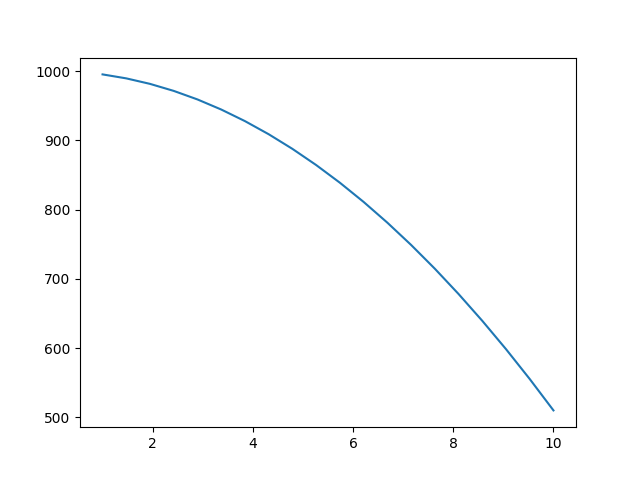
\includegraphics[width=6cm, height=6cm]{/home/jp/kod/py/bin/venv/py3/phx444/labs/lab2/figures/figure1.png}
        % Create a subtitle for the figure.
        \caption{Plotting the Measured values for Magnetic Field}
        % Define the label of the figure. It's good to use `fig:title', so you know that the label belongs to a figure.
        \label{fig:fig_1}
        \end{center}
\end{figure}
I chose to read my data into python as a Pandas DataFrame. In my experience,
pandas is just about the best library to work with heterogeneous data. It's
even able to read an excel file:
\begin{center}
\begin{minipage}[t]{.75\textwidth}
\begin{lstlisting}[frame=tlrb]
xl = pd.ExcelFile(`data/magnetic.xlsx')
df = xl.parse(`Sheet1')
\end{lstlisting}
\end{minipage}
\end{center}
After that, I dropped the non-existent entries off the bottom of the DataFrame
because they're problematic for model fitting. Then, I used the uncerainties
package and a lambda function to propagate error through all of our mass and 
current measurements. I'm not going to copy all of the code here, but the
general syntax follows this form:
\begin{center}
\begin{minipage}[t]{.75\textwidth}
\begin{lstlisting}[frame=tlrb]
<Measurement>= \
    df[<Measurement>].dropna().apply(
        lambda x: ufloat(x, <error>)
    )
\end{lstlisting}
\end{minipage}
\end{center}
Next, for the current menasurements, I looked up the specs for
Keithley's model 2000 6 1/2 digit multimeter. I stared at them for a while.
Then I pestered Brian for a while. Then I stared at the specs some more. Eventually, I
pestered Brian enough that he showed how to read the table. In our case, the current 
has an uncertainty of:
$$(1000 \times I + 3 \times 15) \times 10^{-6}$$
In python, we are able to make use of the pandas data structure and
uncertainties library to propagate this:
\begin{verbatim}
current_error = \
    1000 * df[`current'].dropna() * 10 ** -6 + 3 * 15 * 10**-6

b_cal_current = \
    pd.Series(uarray(df[`current'].dropna(), current_error))
\end{verbatim}
Notice that I have to explicitly turn the result back into a
pandas object. The uarray() method returns a NumPy Array. It would be totally
fine to leave the result as a NumPy object, but syntactically NumPy is slightly
different and Pandas, so it's beneficial to have all objects be the same type.

I was able to fit the curve using the same method as in the data
analysis lab. Specifically, I assumed linearity and fit it with:

\begin{center}
\begin{minipage}[t]{.75\textwidth}
\begin{lstlisting}[frame=tlrb]
def lin_fit(x, a, b):
    return a*x + b

popt, pcov = curve_fit(
                lin_fit, 
                current_values, 
                b_cal_values
            )

b_fit = lin_fit(
    current_values, 
    *popt
)
\end{lstlisting}
\end{minipage}
\end{center}

We learned last lab that residuals are a pretty decent sanity check on the
accuracy of data and models. So let's go ahead and plot the residuals from this
fit:

\begin{center}
\begin{minipage}[t]{.75\textwidth}
\begin{lstlisting}[frame=tlrb]
r_i = b_cal_values - b_fit

plt.errorbar(
    current_values,
    r_i,
    yerr=b_cal_error,
    fmt='o')
\end{lstlisting}
\end{minipage}
\end{center}

And showing this plot, we find that the residuals are actually quite
reasonable. They are clustered around zero and their error bars are easily
visible. Notice that the size of the error bars around zero is quite large.
This makes sense because the current error ought to be similar in magnitude, but
its fractional error will increase:

\begin{figure}[H]
        % Center the figure.
        \begin{center}
        % Include the eps file, scale it such that it's width equals the column width. You can also put width=8cm for example...
        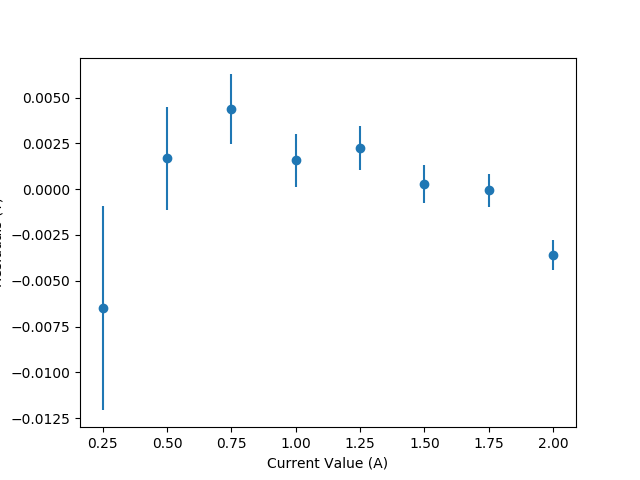
\includegraphics[width=6cm,
        height=6cm]{/home/jp/kod/py/bin/venv/py3/phx444/labs/lab2/figures/figure1b.png}
        % Create a subtitle for the figure.
        \caption{Plotting the residuals as a sanity check}
        % Define the label of the figure. It's good to use `fig:title', so you know that the label belongs to a figure.
        \label{fig:fig_2}
        \end{center}
\end{figure}


\subsection{Magnetic Susceptibility of Samples}
Now, hopefully I've convinced you that the environment between our magnets
houses a magnetic field that is approximately .4 Teslas strong. If I haven't
convinced you yet, try this:

\begin{center}
\begin{minipage}[t]{.75\textwidth}
\begin{lstlisting}[frame=tlrb]
def understand(paper, confused=True):
    if confused:
        read(section_1)
        read(section_2)
        understand(paper)

    return 
\end{lstlisting}
\end{minipage}
\end{center}

%----------------------------------------------------------------------------------------
%   SECTION 4
%----------------------------------------------------------------------------------------
\section{Conclusion}
I love data science. Even if I come off as dry and sarcastic on paper,
there is genuinely nothing that I would rather be up doing until \st{12:46AM}
11:59PM on a given night. I'm really excited for this semester and hope that
there continues to be a focus on learning / utilizing the classic Python
libraries!
\end{document}


